Although vectors in source code within DPC++ should be interpreted as convenience tools that are local to only a single work-item, this chapter on vectors would not be complete without some mention of how SIMD instructions in hardware operate. This discussion is not coupled to vectors within our source code, but provides orthogonal background that will be useful as we progress to the later chapters of this book that describe specific device types (GPU, CPU, FPGA).\par

Modern CPUs and GPUs contain SIMD instruction hardware that operate on multiple data values contained in one vector register or a register file. For example, with Intel x86 AVX-512 and other modern CPU SIMD hardware, SIMD instructions can be used to exploit data parallelism. On CPUs and GPUs that provide SIMD hardware, we can consider a vector addition operation, for example, on an eight-element vector, as shown in Figure 11-13.\par

\hspace*{\fill} \par %插入空行
Figure 11-13. SIMD addition with eight-way data parallelism
\begin{center}
	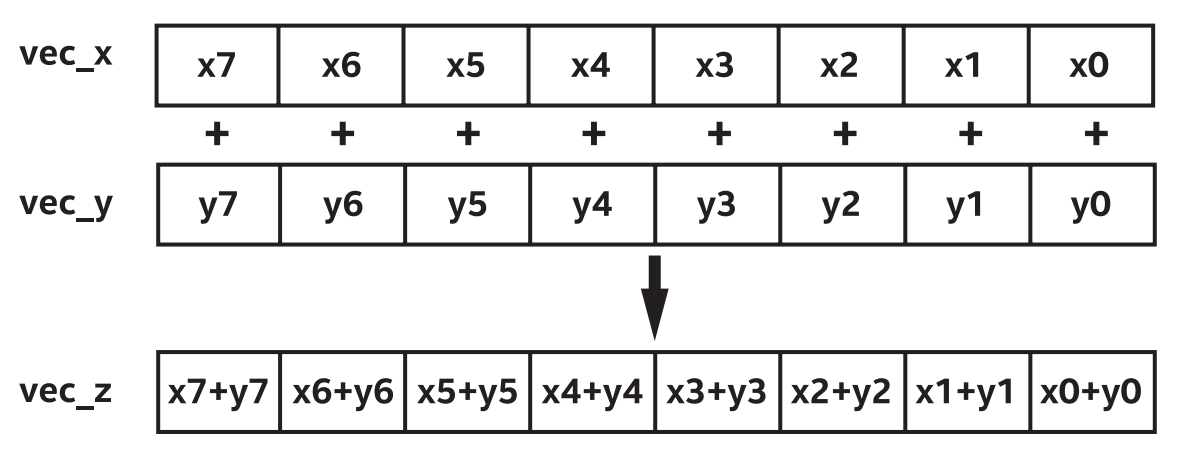
\includegraphics[width=1.0\textwidth]{content/chapter-11/images/2}
\end{center}

The vector addition in this example could execute in a single instruction on vector hardware, adding the vector registers vec\_x and vec\_y in parallel with that SIMD instruction.\par

Exposing potential parallelism in a hardware-agnostic way ensures that our applications can scale up (or down) to fit the capabilities of different platforms, including those with vector hardware instructions. Striking the right balance between work-item and other forms of parallelism during application development is a challenge that we must all engage with, and that is covered more in Chapters 15, 16, and 17.\par













